\documentclass[a4paper,11pt]{jsarticle}

% 数式
\usepackage{amsmath,amsfonts}
\usepackage{bm}
% 画像
\usepackage[dvipdfmx]{graphicx}
% bibTeX
\usepackage[backend = biber,style =apa, sorting =none,]{biblatex}

% 参考文献ファイルのリスト
% \addbibresource{references.bib}

% 等式番号を章ごとに割り振る
\makeatletter
\@addtoreset{equation}{section}
\def\theequation{\thesection.\arabic{equation}}
\makeatother

% ハイパーリンク
\usepackage[dvipdfmx]{hyperref}
\usepackage{pxjahyper}

% listings(ソースコード)
\usepackage{listings}
\usepackage{color}

\definecolor{dkgreen}{rgb}{0,0.6,0}
\definecolor{gray}{rgb}{0.5,0.5,0.5}
\definecolor{mauve}{rgb}{0.58,0,0.82}

\lstset{
language=Python,
basicstyle=\small\sffamily,
numbers=left,
numberstyle=\tiny\color{gray},
keywordstyle=\color{blue},
commentstyle=\color{dkgreen},
stringstyle=\color{mauve},
frame=single,
columns=fullflexible,
showspaces=false,
showstringspaces=false,
tabsize=3
}
\renewcommand{\lstlistingname}{}

\begin{document}

\title{計算機科学実験4 音声 レポート2}
\author{
  京都大学工学部情報学科\\
  計算機科学コース3回生\\
  学生番号: 1029-33-1415\\
  氏名: 安済翔真\\
}
\date{\today}
\maketitle

\tableofcontents
\newpage


\section{機能・プログラム説明}

課題2では音響信号を操作するグラフィカルユーザーインタフェースを作成した。
この章では作成した具体的な機能について説明する。
画面全体は図\ref{fig:work2_app}のようになっている。

\begin{figure}[h]
\centering
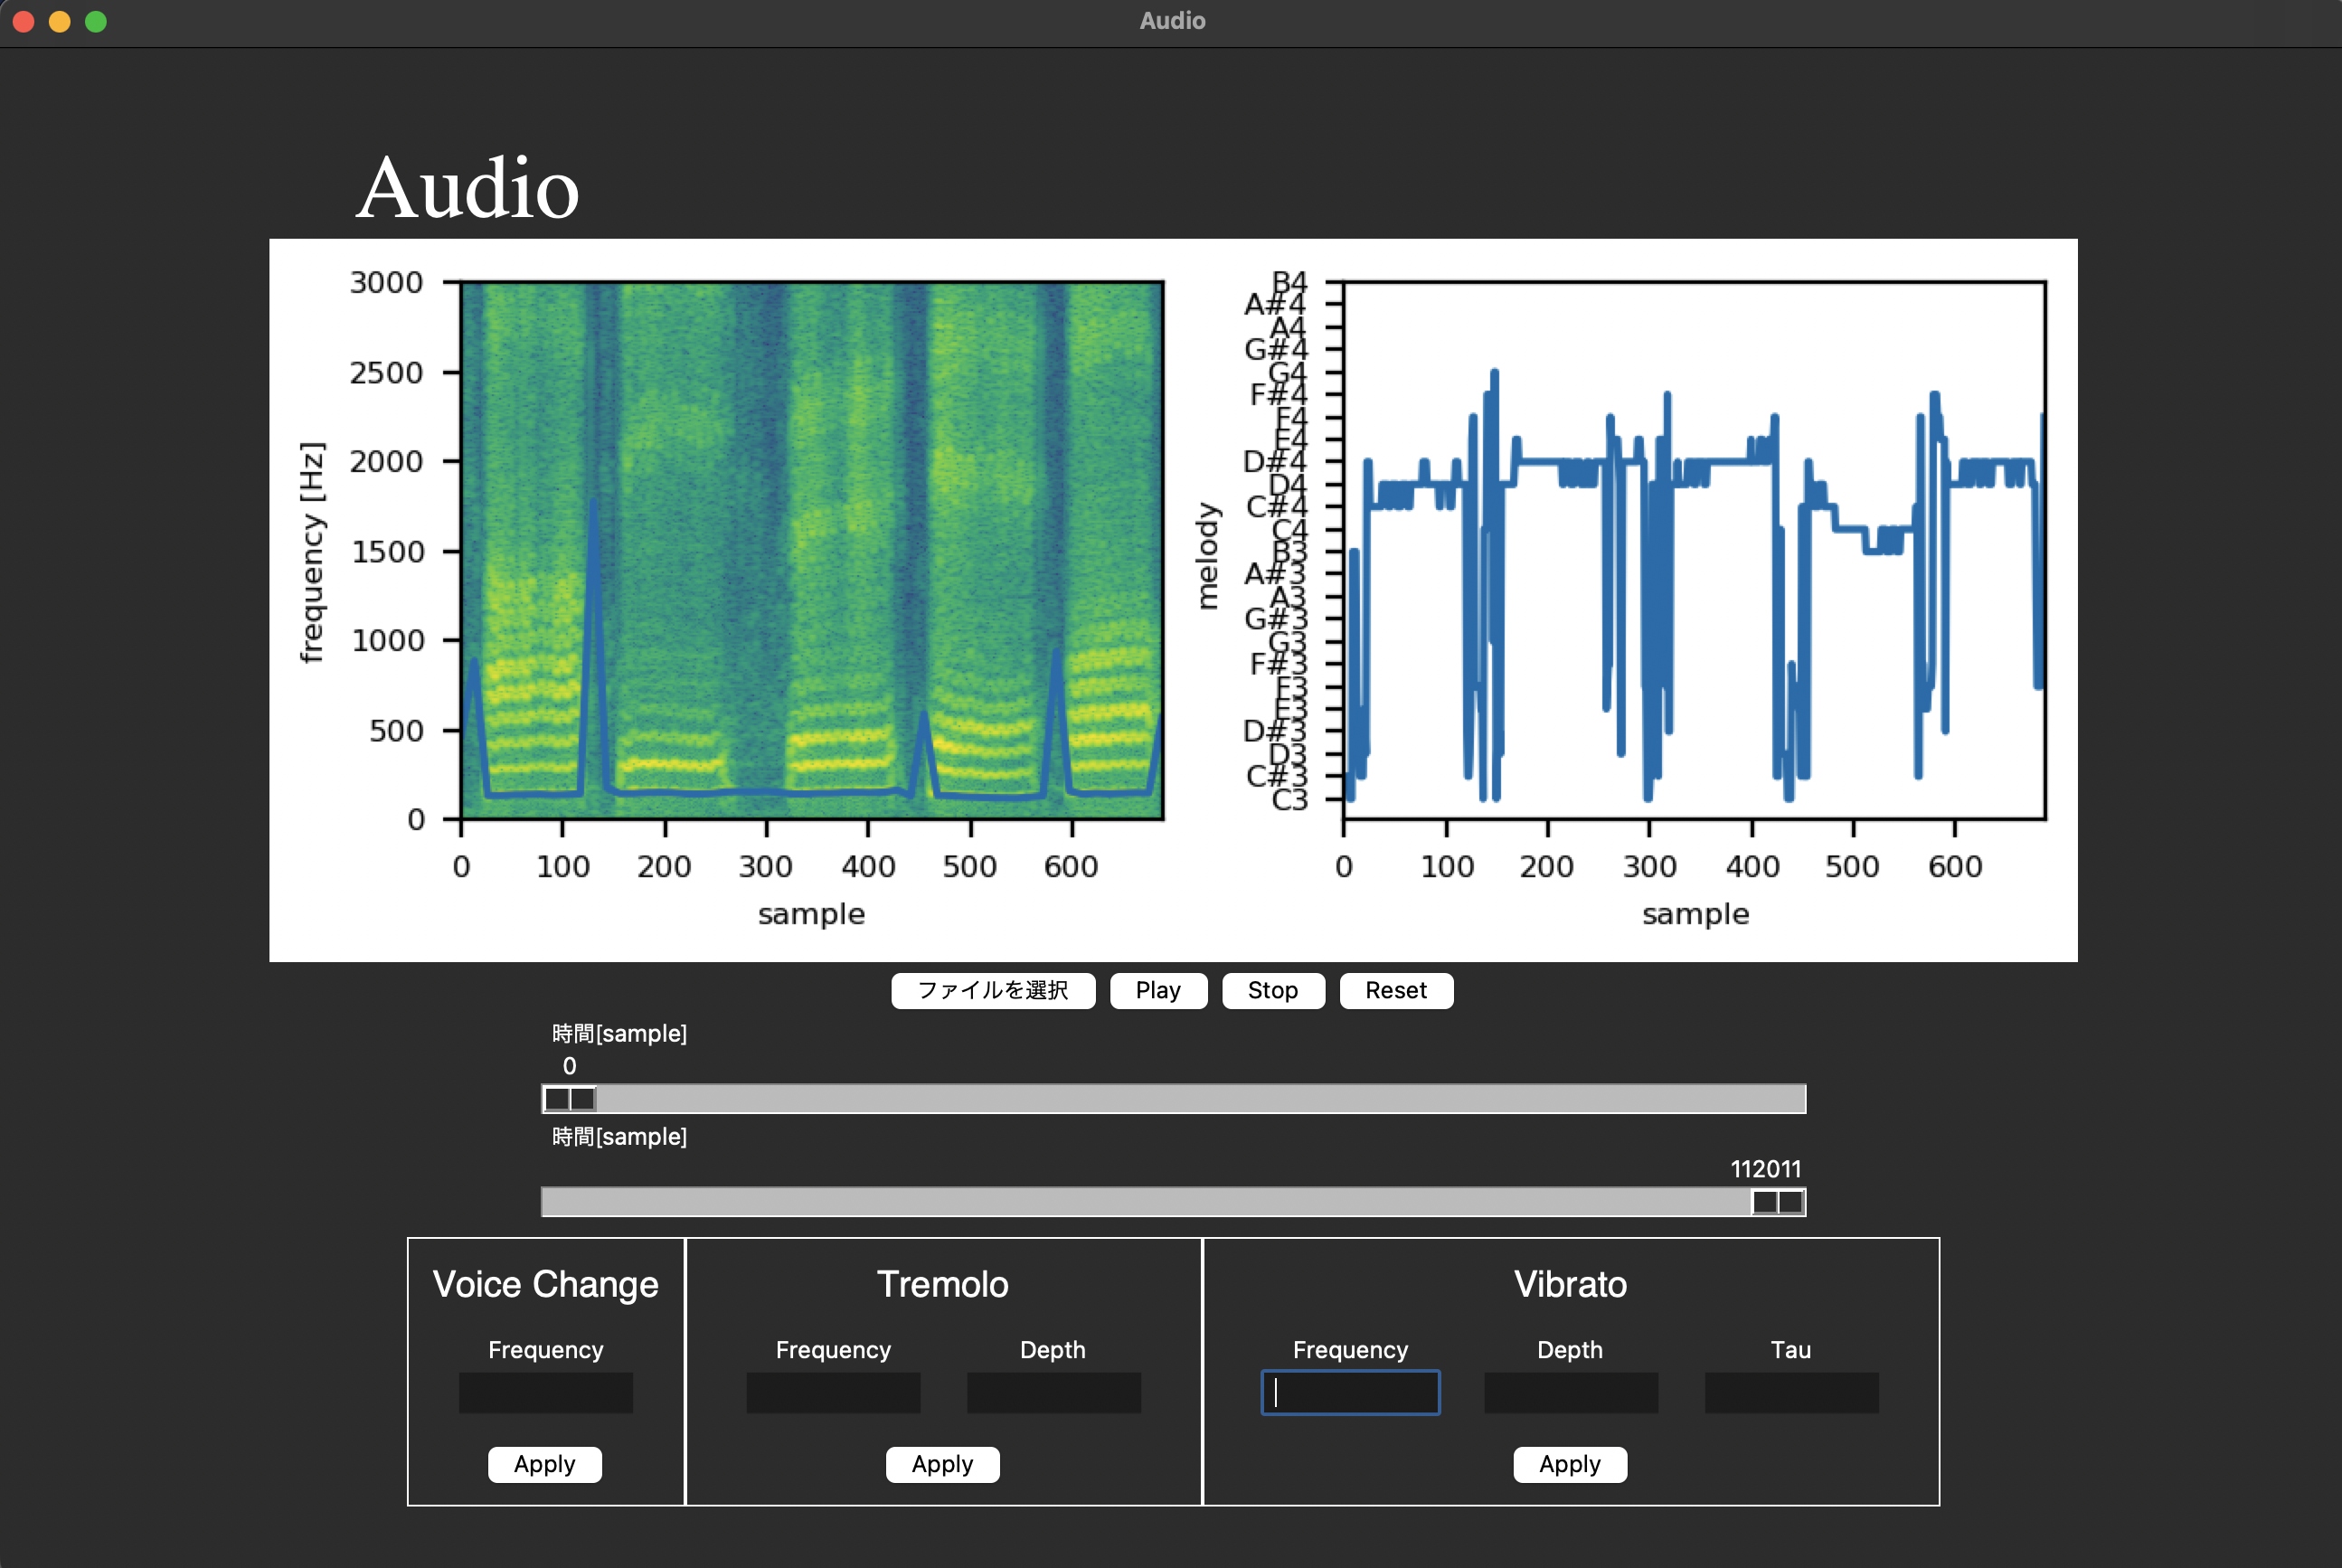
\includegraphics[keepaspectratio, width=13cm]
{./images/work2_app.png}
\caption{画面全体}
\label{fig:work2_app}
\end{figure}

\subsection{ファイル選択}
ファイル選択機能を実装した。ファイル選択ボタン(図\ref{fig:select_file})を押すと、ファイル選択ダイアログが表示される。
選択したファイルを読み取り、操作対象の音声データとして扱う。

\begin{figure}[h]
\centering
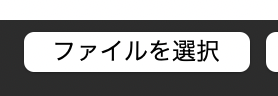
\includegraphics[keepaspectratio, scale = 1.0]
{./images/select_file.png}
\caption{ファイル選択ボタン}
\label{fig:select_file}
\end{figure}

ファイル読み取りのプログラムはコード\ref{code:load_file1}, \ref{code:load_file2}の通りである。
コード\ref{code:load_file1}ではtkinterのfiledialogを用いてファイル選択ダイアログを表示し、
選択したファイル名を取得する。コード\ref{code:load_file2}ではlibrosaを用いて音声データを読み取る。

\begin{lstlisting}[caption=ファイル読み取り1,label=code:load_file1]
  filename = tk.filedialog.askopenfilename()
  self._c.load_file(filename)
\end{lstlisting}

\begin{lstlisting}[caption=ファイル読み取り2,label=code:load_file2]
def load_waveform(filename):
  x, _ = librosa.load(filename, sr=SR)
  return x
\end{lstlisting}

\subsection{ビブラート}
選択したファイルの音声にビブラートをかける機能を実装した。
コード\ref{code:vibrato}はビブラートをかけるプログラムである。
generate\_sinusoid関数は、サンプリング周波数S、周波数F、長さTを引数に取り、
サンプリング周波数Sで周波数Fの正弦波を長さT秒分生成する関数である。
引数に、元の波形、サンプリング周波数S、ビブラートの周波数F、ビブラートの深さD、
ビブラートの遅れ時間$\tau$を取り、次の式に従って波形を変形させた。

\begin{equation}
  \left\{
  \begin{aligned}
    x'_t &= x_{t-\tau(t)} \\
    \tau(t) &= \tau 0 + D \sin(2 \pi F t)
  \end{aligned}
  \right.
\end{equation}

\begin{lstlisting}[caption=ビブラート,label=code:vibrato]
def vibrato(waveform, sampling_rate: int, frequency: float, depth: float, tau: float):
  vibrato_waveform = generate_sinusoid(sampling_rate, frequency, len(waveform) / sampling_rate)
  changed = waveform.copy()
  for i in range(len(waveform)):
    taui = int(tau + depth * vibrato_waveform[i])
    if taui < 0:
      taui = 0
    elif taui >= len(waveform):
      taui = len(waveform) - 1
    changed[i] = waveform[i - taui]
  return changed
\end{lstlisting}

\subsection{ボイスチェンジ}
選択されたファイルの音声にボイスチェンジをかける機能を実装した。
コード\ref{code:voice_change}はボイスチェンジをかけるプログラムである。
sin波を生成して、元の波に乗算することで、ボイスチェンジを実現した。

\begin{lstlisting}[caption=ボイスチェンジ,label=code:voice_change]
def voice_change(waveform, sampling_rate, frequency):
  duration = len(waveform)
  sin_wave = generate_sinusoid(sampling_rate, frequency, duration / sampling_rate)
  sin_wave = sin_wave * 0.9
  return waveform * sin_wave
\end{lstlisting}

\subsection{トレモロ}
選択したファイルの音声にトレモロをかける機能を実装した。
コード\ref{code:tremolo}はトレモロをかけるプログラムである。
次の式で得られる信号を入力音声に乗算することで、トレモロを実現した。

\begin{equation}
  a(t) = 1 + D \sin(2 \pi F t)
\end{equation}


\begin{lstlisting}[caption=トレモロ,label=code:tremolo]
def tremolo(waveform, sampling_rate, frequency, depth):
  tremolo_waveform = generate_sinusoid(sampling_rate, frequency, len(waveform) / sampling_rate)
  changed = waveform * (1.0 + depth * tremolo_waveform)
  return changed / np.max(np.abs(changed))
\end{lstlisting}

\subsection{スペクトログラムの表示}
加工後の音声のスペクトログラムを表示する機能を実装した。
ビブラート、ボイスチェンジ、トレモロの各加工を行うと図が自動で更新され、
加工後の音声のスペクトログラムが表示される。
コード\ref{code:calc_spectrogram}はスペクトログラムを計算するプログラムである。
numpyのhamming関数を用いて窓掛けを行い、FFTを行う。
その後、対数振幅スペクトルを計算し、配列に保存する。

\begin{lstlisting}[caption=スペクトログラム計算,label=code:calc_spectrogram]
def spectrogram(waveform, size_frame, size_shift):
  spectrogram = []
  hamming_window = np.hamming(size_frame)

  for i in np.arange(0, len(waveform) - size_frame, size_shift):
    idx = int(i)
    x_frame = waveform[idx: idx + size_frame]

    # 窓掛けしたデータをFFT
    fft_spec = np.fft.rfft(x_frame * hamming_window)

    # 振幅スペクトルを対数化
    fft_log_abs_spec = np.log(np.abs(fft_spec))

    # 配列に保存
    spectrogram.append(fft_log_abs_spec)
  return spectrogram
\end{lstlisting}

コード\ref{code:show_spectrogram}はスペクトログラムを表示するプログラムである。
matplotlibのimshow関数を用いてスペクトログラムを表示する。
\begin{lstlisting}[caption=スペクトログラム表示,label=code:show_spectrogram]
self.__ax.imshow(
    np.flipud(np.array(spectrogram).T),
    extent=[0, len(spectrogram), 0, SR / 2],
    aspect='auto',
    interpolation='nearest',
)
self.__ax.set_ylim(0, 3000)
\end{lstlisting}

\subsection{基本周波数の表示}
加工後の音声の基本周波数を表示する機能を実装した。
ビブラート、ボイスチェンジ、トレモロの各加工を行うと図が自動で更新され、
加工後の音声の基本周波数が表示される。
コード\ref{code:calc_f0}は基本周波数を計算するプログラムである。
まず、numpyのcorrelate関数を用いて自己相関係数を計算する。
その後、ピークを検出し、ピークのインデックスを取得する。
最後に、ピークのインデックスから基本周波数を計算する。

\begin{lstlisting}[caption=基本周波数計算,label=code:calc_f0]
def get_f0(waveform, sampling_rate):
  autocorr = np.correlate(waveform, waveform, 'full')
  autocorr = autocorr[len(autocorr) // 2:]  # 不要な前半を捨てる

  # ピークを検出
  peak_indices = [i for i in range(len(autocorr)) if is_peak(autocorr, i)]
  peak_indices = [i for i in peak_indices if i != 0]  # 最初のピークは除く

  if len(peak_indices) == 0:
    return 0

  max_peak_index = max(peak_indices, key=lambda index: autocorr[index])

  # 基本周波数を推定
  f0 = sampling_rate / max_peak_index
  return f0
\end{lstlisting}

コード\ref{code:show_f0}は基本周波数を表示するプログラムである。
matplotlibのplot関数を用いて基本周波数を表示する。
スペクトログラムと同じx軸を用いるため、x軸のデータはスペクトログラムのデータを用いる。

\begin{lstlisting}[caption=基本周波数表示,label=code:show_f0]
  x_data = np.linspace(0, len(spectrogram), len(f0s))
  self.__ax.plot(x_data, f0s)
\end{lstlisting}

\subsection{音程の表示}
加工後の音声の音程を表示する機能を実装した。
ビブラート、ボイスチェンジ、トレモロの各加工を行うと図が自動で更新され、
加工後の音声の音程が表示される。
コード\ref{code:calc_pitch}は音程を計算するプログラムである。
nn2hz関数はMIDIノートナンバーを周波数に変換する関数である。
shs関数はスペクトルを用いて音程を計算する関数である。
候補の音程(NOTES)の各周波数について、スペクトルの対数振幅スペクトルを用いて尤度を計算する。
尤度を計算する際は、対象の音程の「倍音」の強さも考慮した。特に、倍音の強さは
0.8の指数関数的な減衰を考慮することで精度が大幅に向上した。

\begin{lstlisting}[caption=音程計算,label=code:calc_pitch]
def nn2hz(nn):
  return 440.0 * 2 ** ((nn - 69) / 12.0)

def shs(spectrum, sample_rate, size_frame):
  likelihood = np.zeros(len(NOTES))
  for i in range(len(likelihood)):
    base_freq = nn2hz(NOTES[i])
    for j in range(1, 16):
      freq = base_freq * j
      fft_idx = int(freq * size_frame / sample_rate)
      likelihood[i] += 0.8**j * np.exp(spectrum[fft_idx])
  return NOTES[np.argmax(likelihood)]

\end{lstlisting}

コード\ref{code:show_pitch}は音程を表示するプログラムである。
matplotlibのplot関数を用いて音程を表示する。
yticksでy軸のラベルを設定している。ラベルの内容はC3からB4までの音程を表示することで、
表示される音程がわかりやすくなるようにした。

\begin{lstlisting}[caption=音程表示,label=code:show_pitch]
  plt.plot(list(map(lambda x: x - NOTES[0], melody)))
  plt.yticks(np.arange(24),
         list(["C3", "C#3", "D3", "D#3", "E3", "F3", "F#3", "G3",
               "G#3", "A3", "A#3", "B3", "C4", "C#4", "D4", "D#4",
               "E4", "F4", "F#4", "G4", "G#4", "A4", "A#4", "B4"])
         )
\end{lstlisting}

\subsection{音声の再生・停止}

加工後の音声を再生・停止する機能を実装した。
コード\ref{code:play}は音声を再生するプログラムである。
既に音声が再生中の場合は、一旦再生を停止してから再度再生をすることで、
同じ音声を連続して再生することができる。

\begin{lstlisting}[caption=音声再生,label=code:play]
  if self.__play_obj is not None:
    self.__play_obj.stop()
  self.__play_obj = self.__wave_obj.play()
\end{lstlisting}

コード\ref{code:stop}は音声を停止するプログラムである。
音声が再生中の場合のみ、音声を停止する。

\begin{lstlisting}[caption=音声停止,label=code:stop]
  if self.__play_obj is None:
    return
  self.__play_obj.stop()
  self.__play_obj = None

\end{lstlisting}

\subsection{表示区間・再生区間の限定}

加工対象の音声の区間を限定する機能を実装した。
選択した区間に対してのみ、ビブラート、ボイスチェンジ、トレモロの各加工が行われる。
コード\ref{code:limit}は表示区間・再生区間を限定するプログラムである。
startの値はendの値より大きくならないようバリデーションを行った。

\begin{lstlisting}[caption=表示区間・再生区間の限定,label=code:limit]
  def set_start(self, start: int):
    if start >= self.__end - self.MIN_SIZE:
      return
    self.__start = start

  def set_end(self, end: int):
    if end <= self.__start + self.MIN_SIZE:
      return
    self.__end = end
\end{lstlisting}

コード\ref{code:show_limit}は区間を限定するUIを表示するプログラムである。
tkinterのScaleを用いて、スライダーのUIを表示している。
このコードにより、図\ref{fig:sliders}のようなUIが表示される。

\begin{lstlisting}[caption=区間を限定するUI,label=code:show_limit]
  self.slider = tk.Scale(
    command=self.__command,
    master=self._frame,
    from_=from_,
    to=to,
    label=u'時間[sample]',
    orient=tk.HORIZONTAL,
    length=700,
    width=15,
  )
\end{lstlisting}

\begin{figure}[h]
\centering
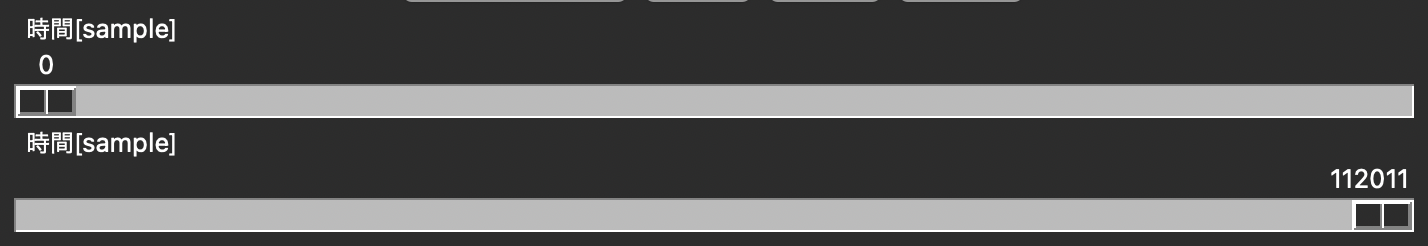
\includegraphics[keepaspectratio, width = 13cm]
{./images/sliders.png}
\caption{区間を限定するUI}
\label{fig:sliders}
\end{figure}

\section{実行例とテスト}
\subsection{ファイル選択}
ファイル選択ボタンを押すと、図\ref{fig:file_select_dialog}
のようなファイル選択ダイアログが表示される。
これにより、ファイル選択ボタンが正しく動作していることが確認できる。

\begin{figure}[h]
\centering
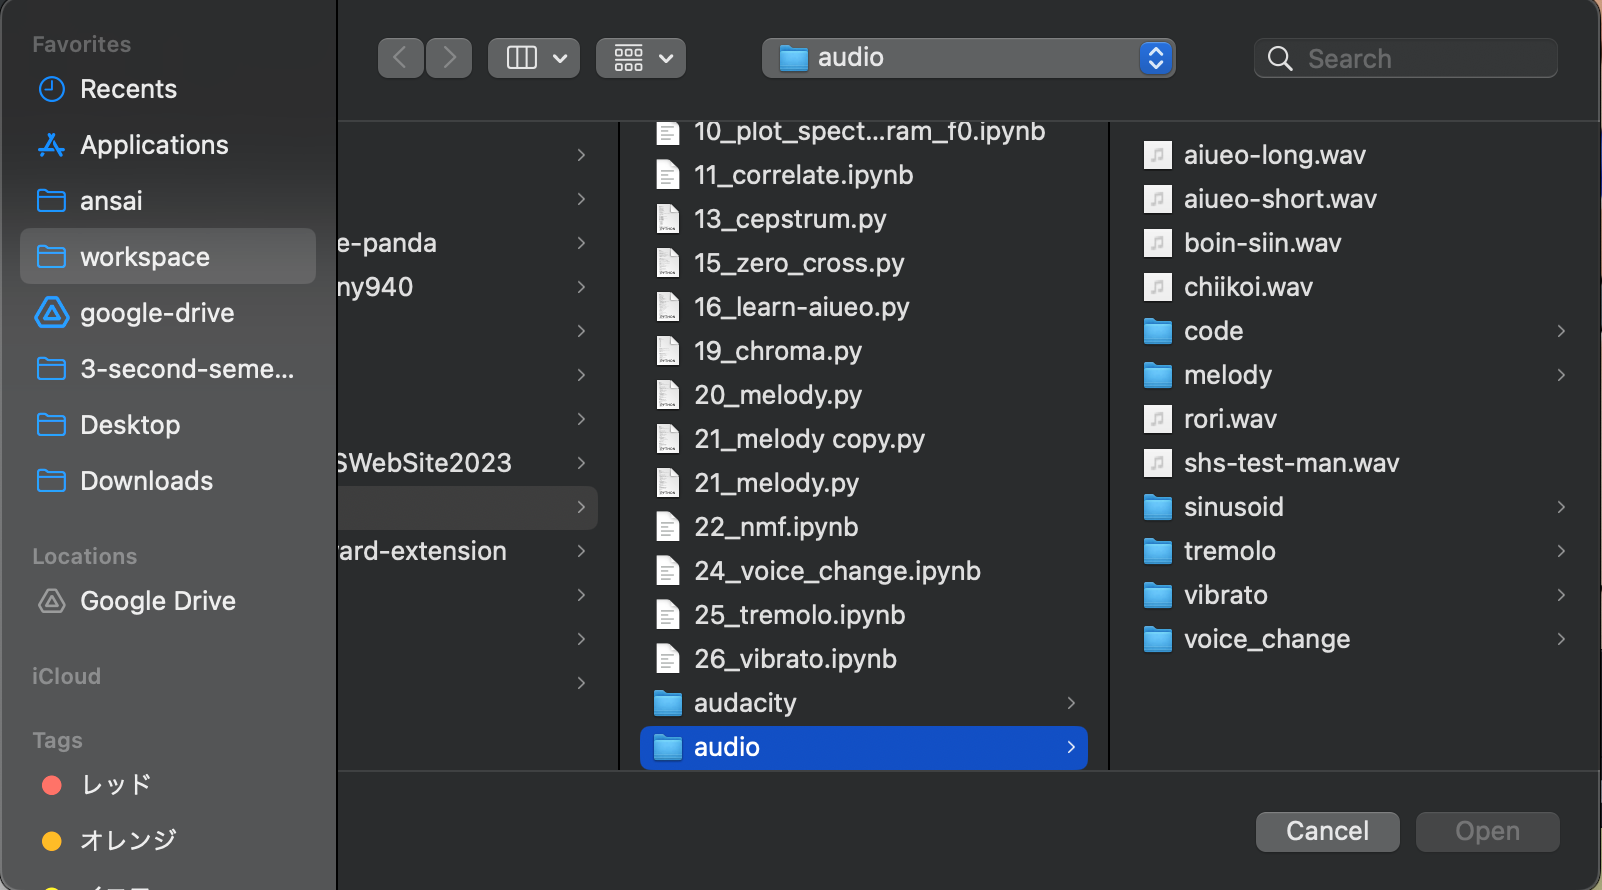
\includegraphics[keepaspectratio, width=13cm]
{./images/file_select_dialog.png}
\caption{ファイル選択ダイアログ}
\label{fig:file_select_dialog}
\end{figure}

\subsection{ビブラート}
ファイルを選択すると、図\ref{fig:vibrato}のようにビブラートの周波数と深さと定数値
を指定するUIが表示される。
frequency, depth, tauの値を入力してApplyボタンを押すと、音声にビブラートがかかることを確認した。

\begin{figure}[h]
\centering
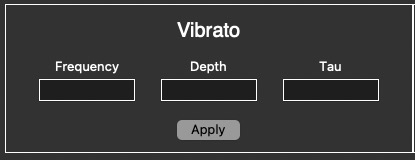
\includegraphics[keepaspectratio, width=13cm]
{./images/vibrato.jpg}
\caption{ビブラートの操作パネル}
\label{fig:vibrato}
\end{figure}

\subsection{ボイスチェンジ}
ファイルを選択すると、図\ref{fig:voice_change}のように
ボイスチェンジの周波数を指定するUIが表示される。
frequencyの値を入力してApplyボタンを押すと、音声にボイスチェンジがかかることを確認した。

\begin{figure}[h]
\centering
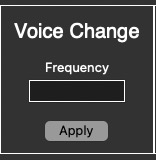
\includegraphics[keepaspectratio, width=13cm]
{./images/voice_change.jpg}
\caption{ボイスチェンジの操作パネル}
\label{fig:voice_change}
\end{figure}

\subsection{トレモロ}
ファイルを選択すると、図\ref{fig:tremolo}のように
トレモロの周波数と深さを指定するUIが表示される。
frequency, depthの値を入力してApplyボタンを押すと、音声にトレモロがかかることを確認した。

\begin{figure}[h]
\centering
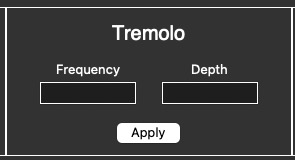
\includegraphics[keepaspectratio, width=13cm]
{./images/tremolo.jpg}
\caption{トレモロの操作パネル}
\label{fig:tremolo}
\end{figure}

\subsection{スペクトログラムの表示}

ファイルを選択すると、図\ref{fig:spectrogram}のようにスペクトログラムが表示される。
また、音声に加工処理を施すと、スペクトログラムが自動で更新される。
図\ref{fig:spectrogram}は「あいうえお」の音声にトレモロをかけた後のスペクトログラムである。
これにより、スペクトログラムが正しく表示されていることが確認できる。

\begin{figure}[h]
\centering
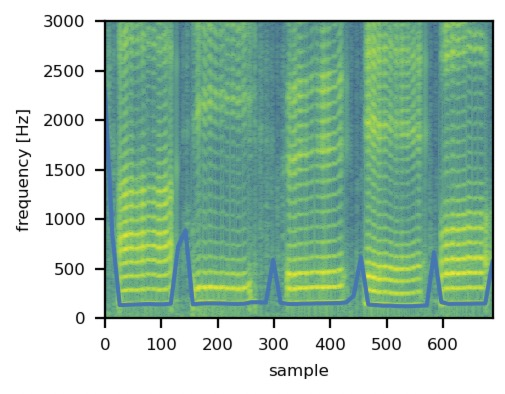
\includegraphics[keepaspectratio, width=13cm]
{./images/spec-tremolo.jpg}
\caption{スペクトログラム}
\label{fig:spectrogram}
\end{figure}

\subsection{基本周波数の表示}

ファイルを選択すると、図\ref{fig:f0}のように基本周波数が表示される。
図\ref{fig:f0}は「あいうえお」の音声にトレモロをかけた後の基本周波数である。
これにより、基本周波数が正しく表示されていることが確認できる。

\begin{figure}[h]
\centering
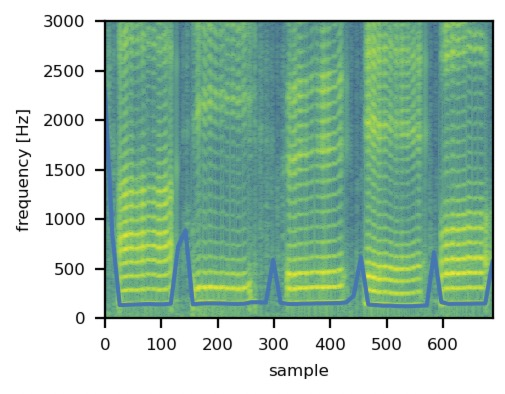
\includegraphics[keepaspectratio, width=13cm]
{./images/spec-tremolo.jpg}
\caption{基本周波数}
\label{fig:f0}
\end{figure}

\subsection{音程の表示}
ファイルを選択すると、図\ref{fig:pitch}のように音程が表示される。
図\ref{fig:pitch}は
\href[]{http://www.sap.ist.i.kyoto-u.ac.jp/members/inoue/le4-audio/}
  {計算機科学実験及演習4 音響信号処理}
のSHS確認用サンプル音声にトレモロをかけた後の音程である。
これにより、音程が正しく表示されていることが確認できる。

\begin{figure}[h]
\centering
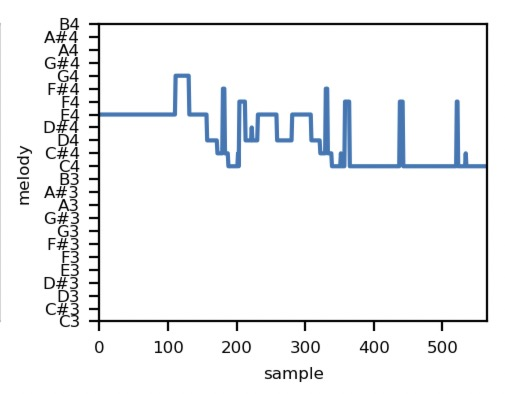
\includegraphics[keepaspectratio, width=13cm]
{./images/melody-tremolo.jpg}
\caption{音程}
\label{fig:pitch}
\end{figure}

\subsection{音声の再生・停止}
ファイルを選択すると、図\ref{fig:play_stop_button}のような再生・停止ボタンが表示される。
再生ボタンを押すと音声が再生され、停止ボタンを押すと音声が停止することを確認した。
音声を加工した後に再生ボタンを押すと、加工後の音声が再生される。
また、再生中に再度再生ボタンを押すと、一旦再生を停止してから再度再生をすることを確認した。

\begin{figure}[h]
\centering
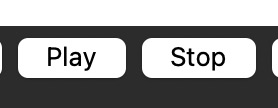
\includegraphics[keepaspectratio, width=13cm]
{./images/play_stop_buttons.jpg}
\caption{再生・停止ボタン}
\label{fig:play_stop_button}
\end{figure}

\subsection{表示区間・再生区間の限定}
ファイルを選択すると、図\ref{fig:sliders}のようなスライダーが表示される。
スライダーで区間を限定すると、加工対象の音声の区間が限定されることを確認した。
また、開始を表すスライダーの値が終了を表すスライダーの値より大きくならないように
なっていることを確認した。

\begin{figure}[h]
\centering
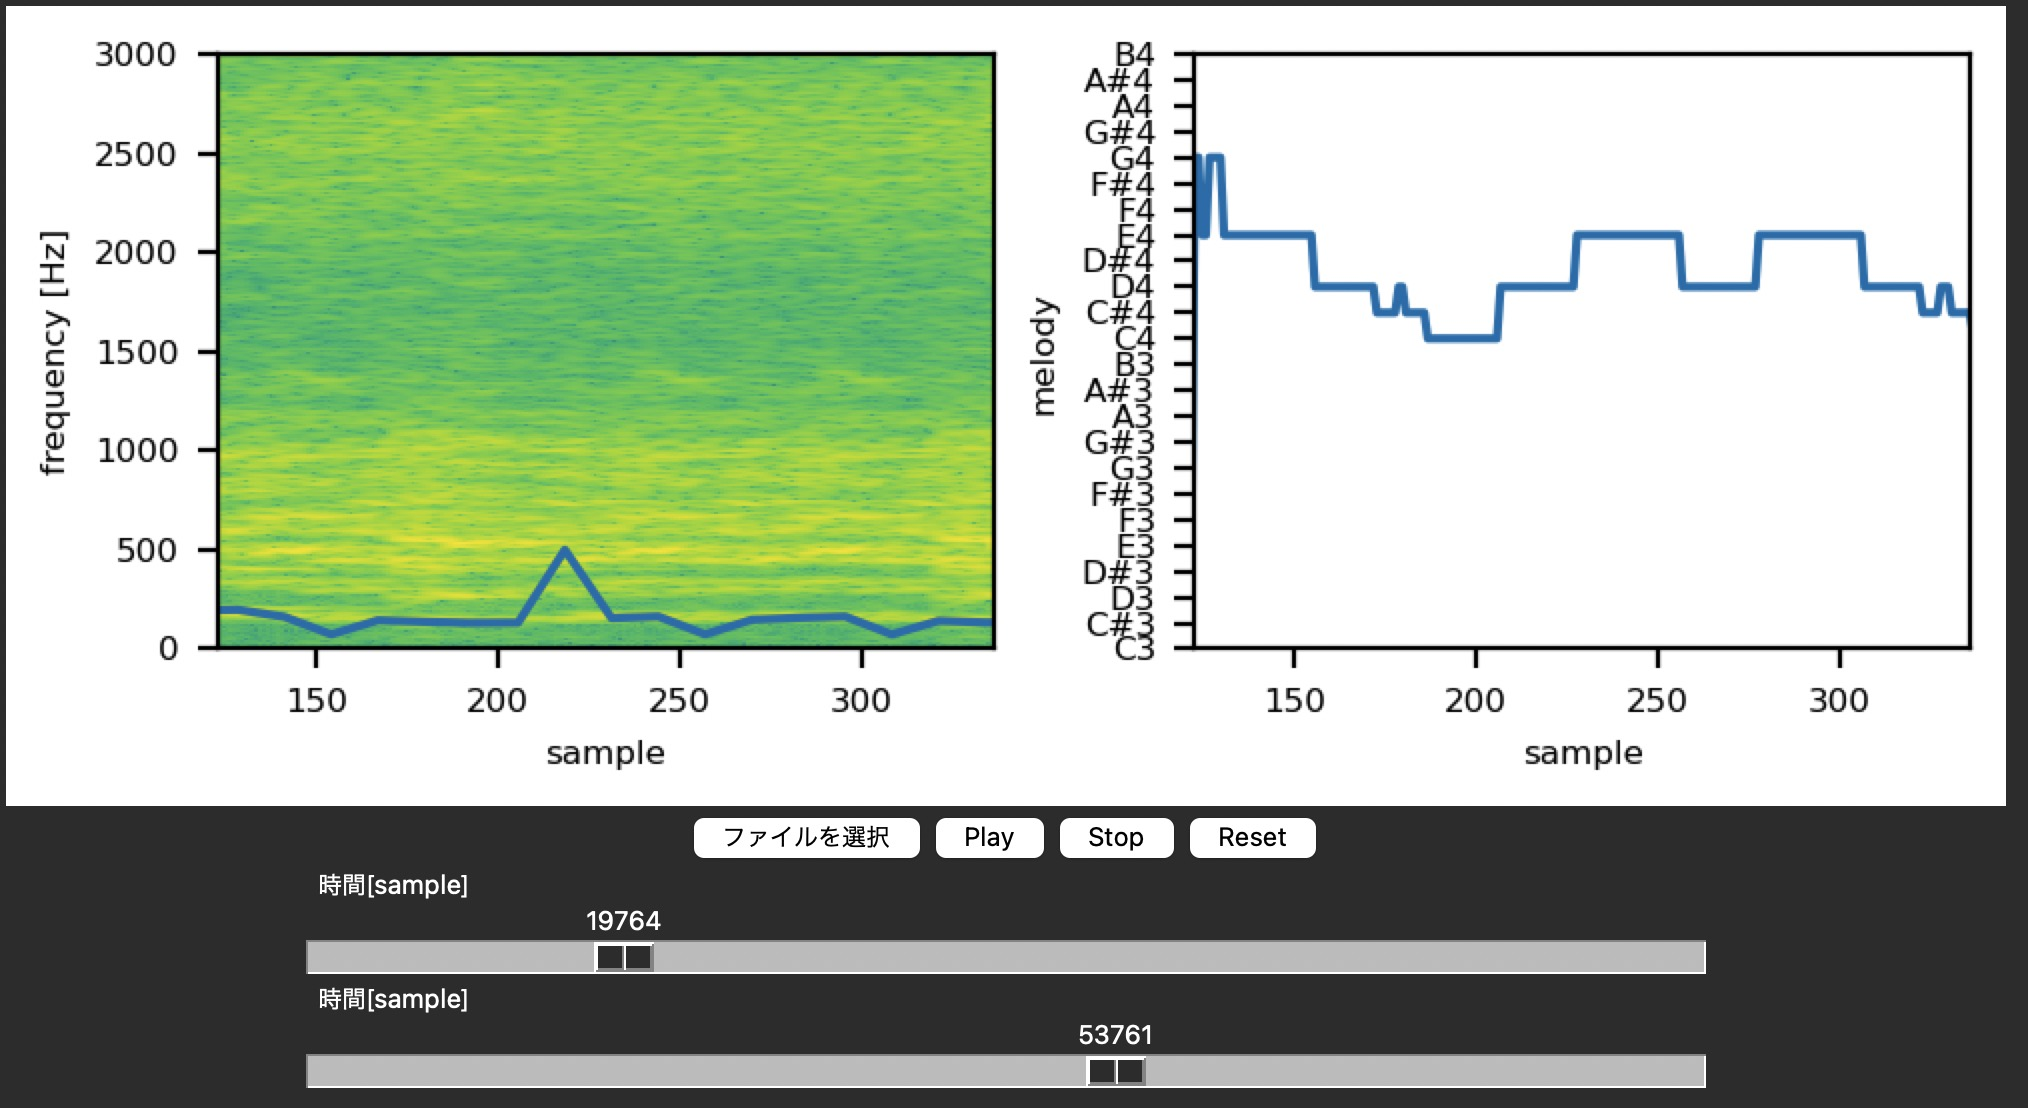
\includegraphics[keepaspectratio, width=13cm]
{./images/filtered_figures.jpg}
\caption{区間を限定した図}
\label{fig:filtered_figures}
\end{figure}

\section{工夫点}
\subsection{ファイル選択機能}
分析対象の音声のファイルは、コードに直接記述するのではなく、ファイルを選択するUIを
用いて選択するようにした。これにより、分析対象の音声を簡単に変更できるようになった。

\subsection{区間選択機能}
加工対象の音声の区間を限定できるように工夫を行なった。
また、startの値がendの値より大きくならないようバリデーションを行った。

\subsection{音程の表示}
音程の図を表示する際に、y軸にはC3からB4までの音程を表示するようにした。
これにより、ノート番号を表示する場合と比べて、表示される音程がわかりやすくなった。

\subsection{音声の再生・停止機能}
音声の再生・停止ボタンを実装した。これにより、加工後の音声をUI上で
実際に確認することが可能になった。

\subsection{コード設計の工夫}
今回作成したGUIアプリでは、コードをcore, view, controllerの3つに分割した。
coreは音声の分析を行う部分、viewはGUIの表示を行う部分、controllerはviewとcoreの
橋渡しを行う部分である。このように分割することで、コードの可読性・保守性を向上させた。

\section{考察}
今回は、音声信号を操作するGUIアプリを作成した。
コードをMVCアーキテクチャに従って整理をすることで、コードの見通しをよくすることができた。
また、音声を加工した時に図が自動的に更新されるといった複雑なUIを作成する勉強になった。
次の課題では音声の分析をリアルタイムで行うGUIシステムを作成する予定である。

% \printbibliography[title=参考文献]

\section{参考文献}
計算機科学実験及演習4 音響信号処理\newline
http://www.sap.ist.i.kyoto-u.ac.jp/members/inoue/le4-audio/


\end{document}
